%%%%%%%%%%%%%%%%%%%%% PACKAGE IMPORTS %%%%%%%%%%%%%%%%%%%%%
\documentclass{article}
\usepackage{import}

\usepackage{amsmath, amsfonts, amsthm, amssymb}
\usepackage{lmodern}
\usepackage{microtype}
\usepackage{fullpage}       
\usepackage{changepage}
\usepackage{hyperref}
\usepackage{blindtext}
\usepackage{subcaption}
\hypersetup{
    colorlinks=true,
    linkcolor=blue,
    filecolor=magenta,      
    urlcolor=blue,
    pdftitle={Overleaf Example},
    pdfpagemode=FullScreen,
    }
\urlstyle{same}

\newenvironment{level}%
{\addtolength{\itemindent}{2em}}%
{\addtolength{\itemindent}{-2em}}

\usepackage{amsmath,amsthm,amssymb}

\usepackage[nooldvoltagedirection]{circuitikz}
\usetikzlibrary{decorations,arrows,shapes}

\usepackage{datetime}
\usepackage{etoolbox}
\usepackage{enumerate}
\usepackage{enumitem}
\usepackage{listings}
\usepackage{array}
\usepackage{varwidth}
\usepackage{tcolorbox}
\usepackage{amsmath}
\usepackage{circuitikz}
\usepackage{verbatim}
\usepackage[linguistics]{forest}
\usepackage{listings}
\usepackage{xcolor}
\renewcommand{\rmdefault}{cmss}


\newcommand\doubleplus{+\kern-1.3ex+\kern0.8ex}
\newcommand\mdoubleplus{\ensuremath{\mathbin{+\mkern-10mu+}}}

\definecolor{codegreen}{rgb}{0,0.6,0}
\definecolor{codegray}{rgb}{0.5,0.5,0.5}
\definecolor{codepurple}{rgb}{0.58,0,0.82}
\definecolor{backcolour}{rgb}{0.95,0.95,0.92}

\lstdefinestyle{mystyle}{
    language=Python,
    basicstyle=\ttfamily\small,
    keywordstyle=\color{blue},
    stringstyle=\color{red},
    commentstyle=\color{green},
    morecomment=[l][\color{magenta}]{\#},
    backgroundcolor=\color{backcolour},   
    breakatwhitespace=false,         
    breaklines=true,                 
    captionpos=b,                    
    keepspaces=true,                 
    numbers=left,                    
    numbersep=5pt,                  
    showspaces=false,                
    showstringspaces=false,
    showtabs=false,                  
    tabsize=2
}

\lstset{style=mystyle}
\setlength{\parindent}{0pt}
\setlength{\parskip}{5pt plus 1pt}

\providetoggle{questionnumbers}
\settoggle{questionnumbers}{true}
\newcommand{\noquestionnumbers}{
    \settoggle{questionnumbers}{false}
}

\newcounter{questionCounter}
\newenvironment{question}[2][\arabic{questionCounter}]{%
    \ifnum\value{questionCounter}=0 \else {\newpage}\fi%
    \setcounter{partCounter}{0}%
    \vspace{.25in} \hrule \vspace{0.5em}%
    \noindent{\bf \iftoggle{questionnumbers}{Question #1: }{}#2}%
    \addtocounter{questionCounter}{1}%
    \vspace{0.8em} \hrule \vspace{.10in}%
}

\newcounter{partCounter}[questionCounter]
\renewenvironment{part}[1][\alph{partCounter}]{%
    \addtocounter{partCounter}{1}%
    \vspace{.10in}%
    \begin{indented}%
       {\bf (#1)} %
}{\end{indented}}

\def\indented#1{\list{}{}\item[]}
\let\indented=\endlist
\def\show#1{\ifdefempty{#1}{}{#1\\}}
\def\IMP{\longrightarrow}
\def\AND{\wedge}
\def\OR{\vee}
\def\BI{\leftrightarrow}
\def\DIFF{\setminus}
\def\SUB{\subseteq}


\newcolumntype{C}{>{\centering\arraybackslash}m{1.5cm}}
\renewcommand\qedsymbol{$\blacksquare$}
\newtcolorbox{answer}
{
  colback   = green!5!white,    % Background colorucyitc,
  colframe  = green!75!black,   % Outline color
  box align = center,           % Align box on text line
  varwidth upper,               % Enables multi line input
  hbox                          % Bounds box to text width
}

\newcommand{\myhwname}{CSE 447 Assignment 3}
\newcommand{\myname}{Sebastian Liu}
\newcommand{\myemail}{ll57@cs.washington.edu}
\newcommand{\mysection}{AB}
\newcommand{\dollararrow}{\stackrel{\$}{\leftarrow}}
%%%%%%%%%%%%%%%%%%%%%%%%%%%%%%%%%%%%%%%%%%%%%%%%%%%%%%%%%%%

%%%%%%%%%%%%%%%%%%% Document Options %%%%%%%%%%%%%%%%%%%%%%
\noquestionnumbers
%%%%%%%%%%%%%%%%%%%%%%%%%%%%%%%%%%%%%%%%%%%%%%%%%%%%%%%%%%%

%%%%%%%%%%%%%%%%%%%%%%%% WORK BELOW %%%%%%%%%%%%%%%%%%%%%%%%
\begin{document}

\begin{center}
    \textbf{Assignment 3} \bigskip
\end{center}

%%%%%%%%%%%%%%%%%%%%%%%% Task 1 %%%%%%%%%%%%%%%%%%%%%%%%M
\begin{question}{1. Baseline Evaluation (15\%)}
    \begin{part}[Q1.1]
        \begin{answer}
            \textbf{Final Average Reward:} 0.6298
        \end{answer}
    \end{part}

    \begin{part}[Q1.2]
        \begin{answer}
            \textbf{Example text \#1:} Young Elijah Wood and Joseph Mazzello are outstanding performers in the film, and they are also the best performers in the film.\\
            \textbf{Example text \#2:} This is one of the best sequels around and a great sequel to the original.\\
            \textbf{Example text \#3:} That's what me and my friends kept asking each other about. I was like, 'What's the best way to do this?' And I was \\
            \textbf{Example text \#4:} "Mame" is a disgrace to many things.\\
            \textbf{Example text \#5:} The Tender Hook, or, Who Killed The President?\\\\

            Sample 1-2 are positive, samples 3 and 5 do not have a clear sentiment, and example 4 has negative sentiments.
            The overall quality of the generation is pretty natural, but it seems to have a hard time generate clear positive sentiments.
        \end{answer}
    \end{part}

    \begin{part}[Q1.3]
        \begin{answer}
            The loop variable is the progress bar which uses tqdm. It keeps track of the evaluation progress as it iterates through the test batches and
            displays the current average reward.
        \end{answer}
    \end{part}
\end{question}

\begin{question}{2. REINFORCE Implementation (20\%)}
    \begin{part}[Q2.1]
        \begin{answer}
            \textbf{Final Average Reward:} 0.8898\\
            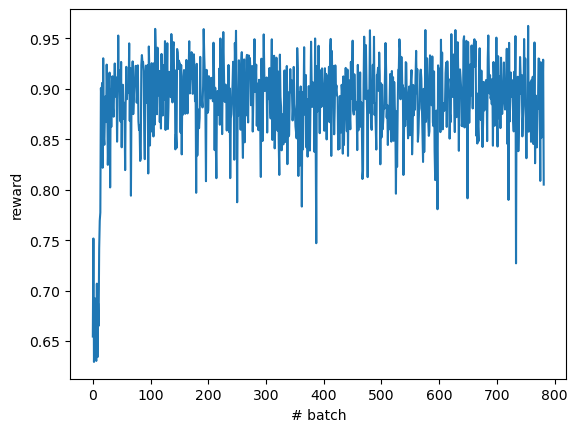
\includegraphics[width=0.8\linewidth]{RL.png}
        \end{answer}
    \end{part}

    \begin{part}[Q2.2]
        \begin{answer}
            \textbf{Example text \#1:} Young Elijah Wood and Joseph Mazzello are outstanding, and I'm pleased to see the world, and I'm pleased to see the world, and\\
            \textbf{Example text \#2:} This is one of the best sequels around and a world, and I'm pleased to see the world, and I'm pleased to see the world,\\
            \textbf{Example text \#3:} That's what me and my friends kept asking each, and I'm pleased to see the world, and I'm pleased to see the world, and\\
            \textbf{Example text \#4:} "Mame" is a disgrace to many things, and I\'m pleased to see the world, and I\'m pleased to see the world, and\\
            \textbf{Example text \#5:} The Tender Hook, or, Who Killed The world, and I'm pleased to see the world, and I'm pleased to see the world,\\\\

            The generations are more positive, but they achieved the positive sentiment by repeating the same positive phrases over and over again, which
            is not natural.
        \end{answer}
    \end{part}
\newpage
    \begin{part}[Q2.3]
        \begin{answer}
            The model tends to reinforce over the same sequence of tokens once they receive a positive reward, and fails to give diverse generations.
            The model also fails to generate coherent sentences, all the example texts are nonsensical.\\
            This is likely due to lack of regularization. The model exploit the reward signal to achieve high reward by repeating the same sequence of tokens and
            ignoring the fluency and coherence of the generated text (reward hacking).
        \end{answer}
    \end{part}

    \begin{part}[Q2.4]
        \begin{answer}
            reset\_model\_optimizer() is used to reinitialize the model and optimizer, which is to make sure that each training run starts with the same initial conditions without any learning from previous runs.
        \end{answer}
    \end{part}

    \begin{part}[Q2.5]
        \begin{answer}
            The shape of log\_probs is torch.Size([32, 30, 50257]), where 32 is the batch size, 30 is the sequence length (max\_length=seed\_token\_length+max\_new\_tokens=10 + 20 = 30), and 50257 is the vocabulary size.
        \end{answer}
    \end{part}

\end{question}

\begin{question}{3. Regularization (15\%)}
    \begin{part}[Q3.1]
        \begin{answer}
            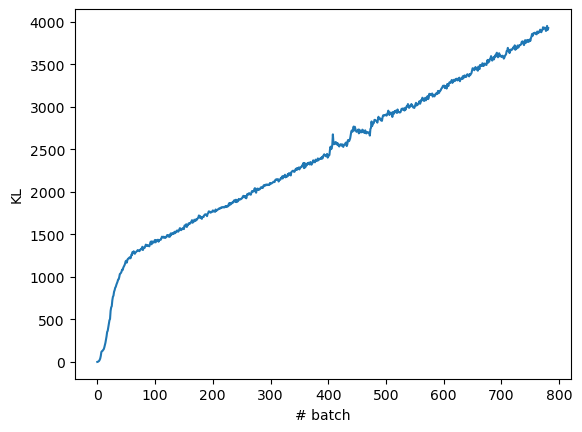
\includegraphics[width=0.5\linewidth]{KL0.png}\\
            The KL-divergence increases over time as training progresses. \\
            This is undesirable because, as the KL-divergence increases, the model is drifting away from the pre-trained distribution (might be an indicator of catastrophic forgetting),
            and the generated text might lose fluency, coherence, or other desirable properties that the model learned from pre-training.
        \end{answer}
    \end{part}

    \begin{part}[Q3.2]
        \begin{answer}
            \textbf{A high $\alpha$ ($\alpha = 10$): } Final Average Reward: 0.6297\\
            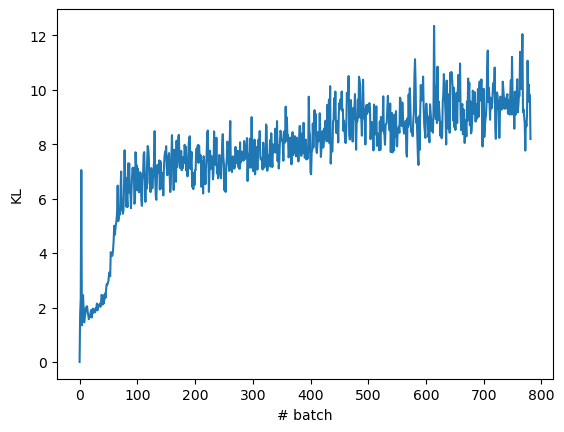
\includegraphics[width=0.5\linewidth]{KL10.png} 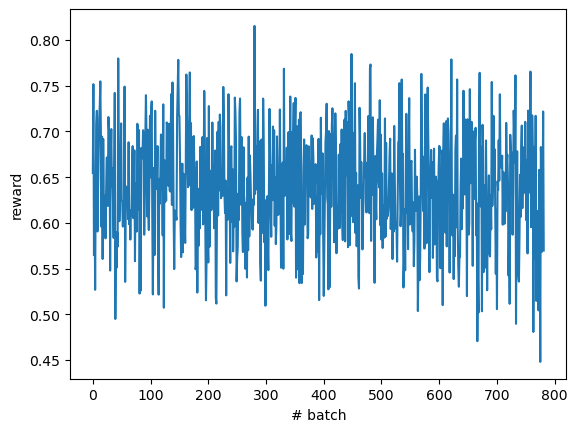
\includegraphics[width=0.5\linewidth]{RW10.png}\\
        \end{answer}
    \end{part}
    \newpage
    \begin{part}[Q3.2 contd.]
        \begin{answer}
            \textbf{Example texts:}\\
                1. Young Elijah Wood and Joseph Mazzello are outstanding performers. They are the best performers in the world. They are the best performers in the world.\\
                2. This is one of the best sequels around and a must-have for any indie game. It’s a must-have for any indie game\\
                3. That's what me and my friends kept asking each other about. I'm a big fan of the show, and I'm a big fan of the\\
                4. "Mame" is a disgrace to many things.\\
                5. The Tender Hook, or, Who Killed The Man, is a series of short stories about the life of a man who was killed by a man\\
           \textbf{Comments:} The quality of the samples are similar to the pretrained model. Sample 1,2, and 5 are positive, sample 4 is negative, and sample 3 is neutral.\\\\
           
           \textbf{A low $\alpha$ ($\alpha = 0.001$): } Final Average Reward: 0.8756\\
            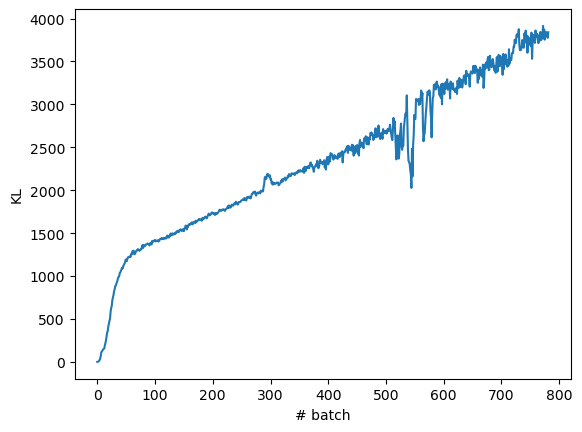
\includegraphics[width=0.5\linewidth]{KLT2.png} 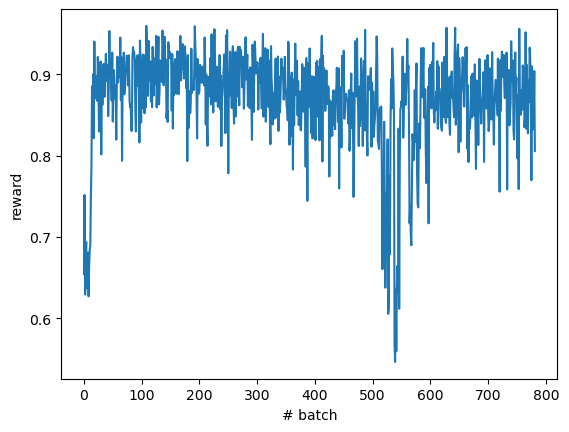
\includegraphics[width=0.5\linewidth]{RW0.001T2.png}\\
            \textbf{Example texts:}\\
            1. Young Elijah Wood and Joseph Mazzello are outstanding world, and I'm pleased to see the world, and I'm pleased to see the world,\\
            2. This is one of the best sequels around and a, and I'm pleased to see the world, and I'm pleased to see the world, and \\
            3. That's what me and my friends kept asking each world, and I'm pleased to see the world, and I'm pleased to see the world,\\
            4. "Mame" is a disgrace to many things world, and I\'m pleased to see the world, and I\'m pleased to see the world, \\
            5. The Tender Hook, or, Who Killed The world, and I'm pleased to see the world, and I'm pleased to see the world, \\
            \textbf{Comments:} The quality of the generations are similar to the un-regularized model. The generation are all positive, but they are not natural and have many repetitions.\\
        \end{answer}
    \end{part}
    \newpage
    \begin{part}[Q3.2 contd.]
        \begin{answer}
            I tried ~20 different $\alpha$ values, but wasn't able to find a good value that get a $\ge 0.8$ reward while getting natural text.
            However, I do found a general trend of high $\alpha$ values tend to perform more similar to the original pre-trained model, but the reward is lower, and low $\alpha$ values tend to perform more similar to the un-regularized model, but the reward is higher.\\\\
            The following is the best model I found which generates reasonably natural texts with pretty good amount of positive sentiments (judged by me):\\
            \textbf{Final Average Reward:} 0.6869\\
            \textbf{ $\alpha = 0.5$}\\
            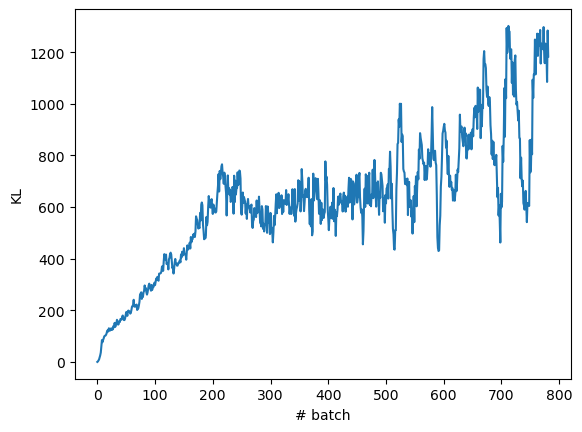
\includegraphics[width=0.5\linewidth]{KL0.5.png} 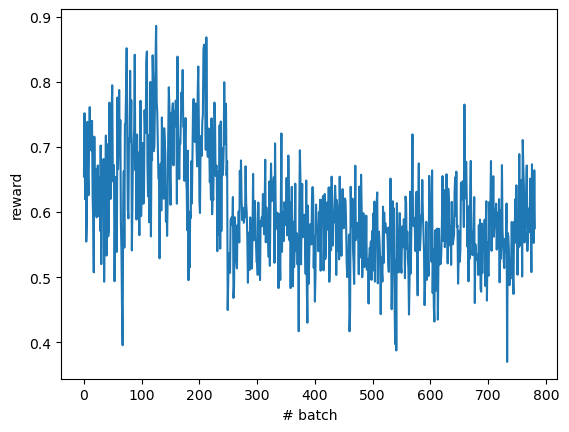
\includegraphics[width=0.5\linewidth]{RW0.5.png}\\
            \textbf{Example texts:}\\
            1. Young Elijah Wood and Joseph Mazzello are outstanding musicians, and they're still getting closer to the music of the 1970s. They're still getting \\
            2. This is one of the best sequels around and a lot of them, but I'm not sure why they're so good. I think they're going \\
            3. That's what me and my friends kept asking each other about their experiences with the game. I've always been fascinated by the game, but I've \\
            4. "Mame" is a disgrace to many things: The Simpsons, which is a great example of how badly flawed the Simpsons were. But there\'s \\
            5. The Tender Hook, or, Who Killed The Beatles, is a fascinating collection of modern music. It is a fascinating collection of music, and it \\

            \textbf{Comments:} The quality of the generations lie in between the high and low $\alpha$ models. Sample 1, 2, 3 and 5 are positive, sample 4 is negative (but it did try to use the word "great" which is generally a positive word).
            The generations are also much more natural and coherent than the high $\alpha$ models, but still not as good as the original pre-trained model.
        \end{answer}
    \end{part}

    \begin{part}[Q3.3]
        \begin{answer}
            One limitation is that both model have high variance in loss and reward, which makes it hard to tune the hyperparameters and the the training is very unstable (might be because the reward signal is sparse).
            One possible solution is to use a baseline function to normalize the rewards or scales the rewards towards a center value, which can reduce the variance and make the training more stable.
        \end{answer}
    \end{part}

    \begin{part}[Q3.4]
        \begin{answer}
            The REINFORCE loss is computed over the 20 tokens (tokens 11...30) generated by the model in response to the seed. The goal of the model is to maximize the expected reward by generating the 20 tokens with the given seed.
            Since first 10 tokens is the fixed seed (i.e. not part of the model's output), so the loss is not computed over the first 10 tokens.
        \end{answer}
    \end{part}

\end{question}

\begin{question}{4. DPO Implementation (35\%)}
    \begin{part}[Q4.1]
        \begin{answer}
            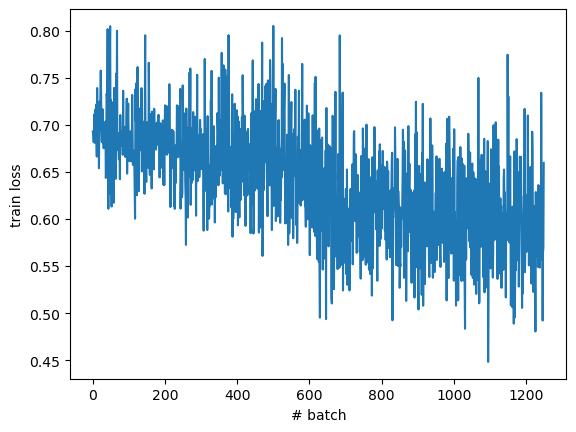
\includegraphics[width=0.8\linewidth]{DPO.png}\\
            \textbf{Average Loss on Test Set:} 0.6552
        \end{answer}
    \end{part}

    \begin{part}[Q4.2]
        \begin{answer}
            \textbf{Final Average Reward:} 0.6466 \\
            The reward for the DPO model is ~0.25 lower than the REINFORCE model.
            One possible reason is that the DPO model is more stable and less likely to exploit the reward signal to achieve high reward by repeating the same sequence of tokens
            and ignoring the fluency of the generated text (reward hacking).
            Another possible reason is that because of the small amount of data and limitation of the pretrained model, the DPO model is not able to learn a good policy to generate high reward text using the given hyperparameters.
        \end{answer}
    \end{part}
\newpage
    \begin{part}[Q4.3]
        \begin{answer}
            \textbf{Example texts:} \\
            1. Young Elijah Wood and Joseph Mazzello are outstanding performers in the film, and they are also the best performers in the film.\\
            2. This is one of the best sequels around and a great sequel to the original.\\
            3. That's what me and my friends kept asking each other about. I was like, 'What's the best way to do this?' And I was \\
            4. "Mame" is a disgrace to many things.\\
            5. The Tender Hook, or, Who Killed The President? \\\\
            \textbf{Comments:} Sample 1 and 2 are positive, sample 4 is negative, and sample 3 and 5 do not have a clear sentiment. The generation are not more positive
            than the original pre-trained model. Actually, the generations are the same as the original pre-trained model.

        \end{answer}
    \end{part}

    \begin{part}[Q4.4]
        \begin{answer}
          \textbf{Experiment 1 ($\beta = 0.1$):} Test Loss: 0.6764, Final Average Reward: 0.6526 \\
          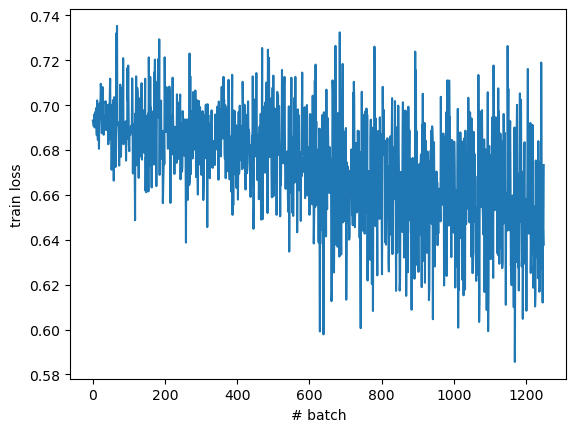
\includegraphics[width=0.5\linewidth]{DPO0.1.png}\\\\
        \textbf{Experiment 2 ($\beta = 0.25$):} Test Loss: 0.6613, Final Average Reward: 0.6500 \\
        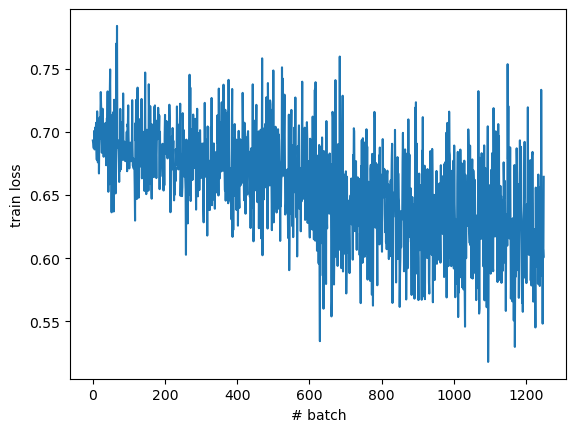
\includegraphics[width=0.5\linewidth]{DPO0.25.png} \\
        \end{answer}
    \end{part}
\newpage
    \begin{part}[Q4.4 contd.]
        \begin{answer}
            \textbf{Experiment 3 ($\beta = 0.175$):} Test Loss: 0.6670, Final Average Reward: 0.6513 \\
            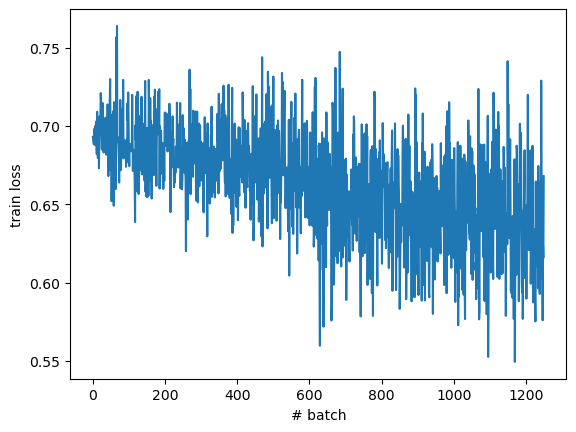
\includegraphics[width=0.5\linewidth]{DPO0.175.png} \\\\

            \textbf{Comments:} The best setup in terms of test loss among the three experiments is $\beta = 0.25$, but the reward is the lowest among the three.
            As we can see from the data of the three experiments, the higher the $\beta$, the lower the test loss, but the lower the reward. This is probably because the higher the $\beta$, the more the model is regularized
            and the less likely the model is to exploit the reward signal.
        \end{answer}
    \end{part}

    \begin{part}[Q4.5]
        \begin{answer}
            \( \sigma \) is used to squash the log probability ratios into the range between 0 and 1 which can help the loss not diverge when the differences between log probs. It can help regularize the model and make the training more stable.
        \end{answer}
    \end{part}

    \begin{part}[Q4.6]
        \begin{answer}
            The main differences/advantages of DPO are that DPO optimizes for human preferences while avoiding reinforcement learning, and DPO doesn't require external reward model (the DPO model is the reward model).
            Also, DPO is more stable and less likely to exploit the reward, because the examples are weighted by how much higher the implicit reward model rates the dispreferred completions, scaled by $\beta$.
        \end{answer}
    \end{part}
\end{question}

\begin{question}{5. GPT-4 Capability Forecast (15 \%)}
    \begin{part}[Q5.1]
        \begin{answer}
            \textbf{Accuracy:} 64.29\% \\
            \textbf{Log loss:} 1.056
        \end{answer}
    \end{part}

    \begin{part}[Q5.2]
        \begin{answer}
            \begin{enumerate}
                \item I was expecting GPT-4 could do things that seemed straightforward for me, like win a tic-tac-toe game, draw "hello" in ascii, and the birthday question but it couldn't do any of that.
                I wan't expecting it to solve some complex questions that took me a while to understand (the car cluster problem, card deck problem, etc.), but it did solve them.
                \item One pattern is that the model struggles with the tasks that don't present clear semantic information in the question or answer. For example, interpreting a tic-tac-toe board represented by characters is challenging for GPT-4 because it can't visualize the board's layout, and
                without the visual understanding of the layout, it is hard to generate the correct answer. Similarly, without being able to have the visual information about the ascii output, it's hard for the model to judge the correctness of the output.
                One potential reason for this could be the lack of semantic continuity in the question or answer. Since the model generate the next token base on the previous tokens, it's hard for the model to generate the correct answer without clear semantic information in the tokens it generates.

                \item I think I'm less confident about GPT-4 to solve my task after taking the quiz. Because the correctness of the answer from GPT-4 is quite unpredictable, and GPT-4 is also overly confident about its wrong answers.
                \item I envision future models to be multi-sensory, capable of learning and decision-making based on diverse inputs like light, sound, text, smell, taste, and touch. It would be cool if they can
                receive information from the environment like a human. It is important because currently the model is trained on a large amount of human generated data, which can be biased or not representative of the real world.
                If the model can observe the world objectively and make decisions based on these observations, it might be able to produce better and more accurate outputs. To make that happen,
                future GPT-x models would need many many more GPUs or a new type of hardware to handle the increased complexity and amount of input information, and potentially new paradigms of multi-modal learning.
            \end{enumerate}
        \end{answer}
    \end{part}
\end{question}
\begin{question}{Acknowledgement}
   
    \begin{answer}
        This assignment was completed by Sebastian Liu.
        ChatGPT 3.5 were used as a human collaborator to ask conceptual questions about RL, DPO, expected correlations between different hyperparameters, the internals
        of different PyTorch functions, and how to train the models locally using Mac's gpu.
    \end{answer}

\end{question}
\end{document}

